\documentclass[a4papper, 10pt]{article}

\usepackage[utf8]{inputenc}
\usepackage[T1]{fontenc}
\usepackage[normalem]{ulem}
\usepackage[british]{babel}
\usepackage{graphicx}
\usepackage{caption}
\usepackage{subcaption}
\usepackage{enumerate}
\usepackage{array}
\usepackage{amsmath,amssymb,mathrsfs}
\usepackage{url}
\usepackage{fullpage}
\usepackage[table]{xcolor}
\usepackage{placeins} 

\definecolor{light-gray}{gray}{0.85}
%\newcolumntype{M}[1]{>{\raggedright}m{#1}}
\newcolumntype{M}[1]{>{\centering\arraybackslash}m{#1}} % To center text in table

\title{Report: OKF4 electrical validation}
\author{Benjamin Boitrelle}
\date{March 2016}

\begin{document}

  \maketitle
  
  %tableofcontents
  
  %\section{Alignment and bounding inspection}:
  \section{Electrical tests}
  \subsection{Auxiliary board}
  
  Some parameters of the auxiliary board are measured (without any module connected).
  \begin{itemize}
    \item Consumption: 343 mA
    \item $V_{clp} \ = \ 2.28 \ V$
    \item $V_{DD_D} \ = \ 3.35 \ V$
    \item $V_{DD_A} \ = \ 3.35 \ V$
  \end{itemize}
  
  \subsection{AM03 smoke test}
  
  First smoke test done without changing the value of  $V_{clp}$, $V_{dd_D}$ of $V_{dd_A}$:
  \begin{itemize}
    \item POWER ON: 608 mA
    \item RESET: 42 mA
    \item ALL: 659 mA
    \item READ: 659 mA mA with 955 errors 
    \item START: 1145 mA 
  \end{itemize}
  
  Parameters of the auxiliary board measured after connecting the module:
  
  \begin{center}
    \begin{tabular}{ c c c}
    \hline %------------------------
      & Voltages without module (V) & Adjusted voltages (V) \tabularnewline
    \hline %------------------------
    \hline %------------------------
    $V_{clp}$ & 2.28 & 2.15 \tabularnewline
    $V_{dd_D}$ & 3.15 & 3.32 \tabularnewline
    $V_{dd_A}$ & 3.24 & 3.35 \tabularnewline
    \end{tabular}
  \end{center}
  
  \section{Calibration}
  
  \subsection{Oscilloscope output}
  
  The sensor number 2 was disconnected $\Rightarrow$ only 5 sensors are working.
  
  \begin{center}
    \begin{tabular}{c c c c c c c}
      \hline %%%%%%%%%%%%%%%%%%%%%%%
        & Chip 1 & Chip 2 & Chip 3 & Chip 4 & Chip 5 & Chip 6 \tabularnewline 
      \hline %%%%%%%%%%%%%%%%%%%%%%%
      \hline %%%%%%%%%%%%%%%%%%%%%%%
      REST/JTAG & OK & \cellcolor{red}Disconnected & OK & OK & OK & OK  \tabularnewline
      HEADER/TRAILER & OK & \cellcolor{red}Disconnected & OK & OK & OK & OK \tabularnewline
      Pixels & Closed & \cellcolor{red}Disconnected & OK & OK & OK & Closed \tabularnewline
      \hline %%%%%%%%%%%%%%%%%%%%%%%
    \end{tabular}
  \end{center}
  
  \subsection{DAQ calibration}
  
    \subsubsection{Chip 6}
  
    Few pixels are opened on the sub-matrix D.
  
    \begin{itemize}
  
    \item Estimation of the "middle points":
    \begin{center}
    \begin{tabular}{ c c c c c }
      \hline %-------------------------------------------------------------------------------------
      \rowcolor{light-gray} $V_{ref_2}$  &   $V_{ref_{1A}}$  &   $V_{ref_{1B}}$  &   $V_{ref_{1C}}$  &   $V_{ref_{1D}}$  \tabularnewline
      \hline %-------------------------------------------------------------------------------------
      \hline %-------------------------------------------------------------------------------------
      98        &        162        &         158       &       100         &        118        \tabularnewline
      \hline %-------------------------------------------------------------------------------------
    \end{tabular}
    \end{center}

    \begin{figure}[!h]
      \begin{center}
        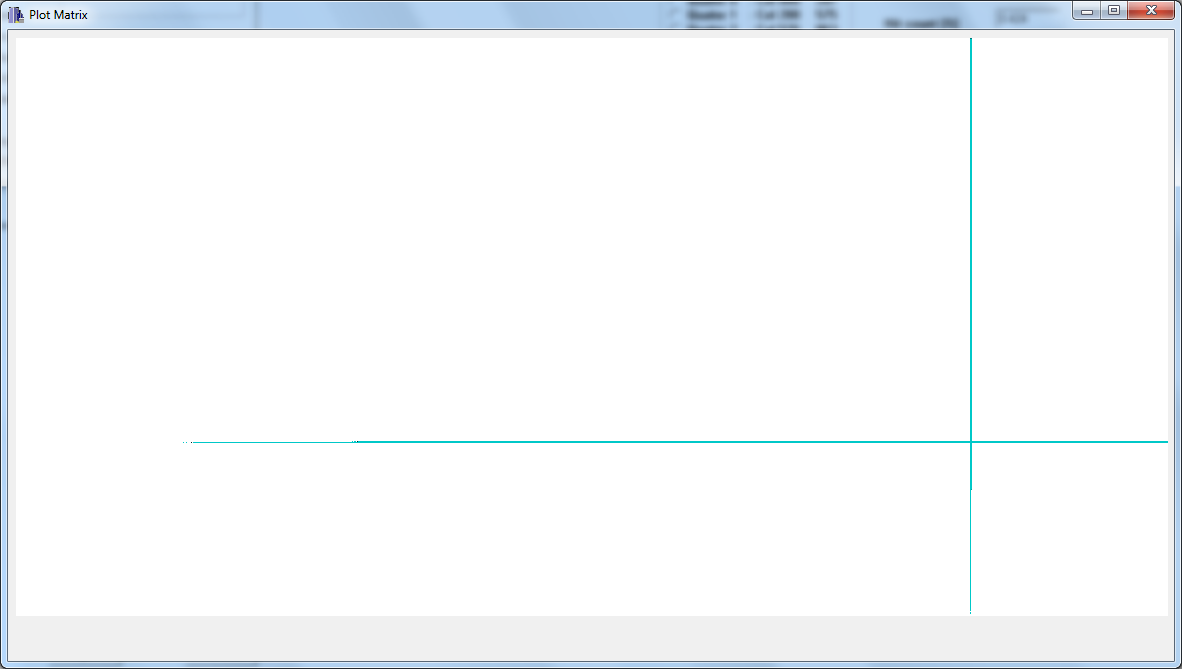
\includegraphics[width = 12cm]{Pictures/Chip6/discri_255.png}
        \label{fig:discri0_chip6}
        \caption{Discriminators output for thresholds set to 255. They are two lines opened and four columns on submatrix D.}
      \end{center}
    \end{figure}
  
    \item Discriminators calibration:
    \begin{center}
    \begin{tabular}{ M{1.3cm} M{1.3cm} M{1.3cm} M{1.3cm} M{1.3cm} M{1.3cm} M{1.3cm} M{1.3cm} M{1.3cm} }
      \hline %-------------------------------------------------------------------
      \rowcolor{light-gray} $V_{ref1_A}$ START  & $V_{ref1_B}$ START & $V_{ref1_C}$ START & $V_{ref1_D}$ START & $V_{ref2}$ & $V_{ref1_A}$ STOP & Step & Event nb / step & Number of Runs \tabularnewline
      \hline %-------------------------------------------------------------------
      \hline %-------------------------------------------------------------------
      134  &  130  &   72  &  90  &  98  &  190  &  2  &  500  &  29  \tabularnewline
      \hline %-------------------------------------------------------------------
    \end{tabular}
    \end{center}

    \item Temporal noise, fixed pattern noise and offset:

            \begin{center}
              \begin{tabular}{ c c c c }
                \hline %----------------------------
         \rowcolor{light-gray}         Matrix  &  TN   &  FPN  &  Offset  \tabularnewline
                \hline %----------------------------
                \hline %----------------------------
                    A     & 1.035 & 0.603 & 0.550    \tabularnewline
                \hline %----------------------------
                    B     & 0.965 & 0.268 & 0.539   \tabularnewline
                \hline %----------------------------
                    C     & 0.980 & 0.595 & 0.476   \tabularnewline
                \hline %----------------------------
                    D     & 1.058 & 0.528 & 0.961    \tabularnewline
                \hline %----------------------------
              \end{tabular}
            \end{center}

    \item Estimation of the fake hit rate ("middle points" thresholds + 20 uadc): $1.66 10^{-3}$ hits/frame/pixels. 
  
    \end{itemize}

    \subsubsection{Chip 5}
  
    \begin{itemize}
  
    \item Estimation of the "middle points":
    \begin{center}
    \begin{tabular}{ c c c c c }
      \hline %-------------------------------------------------------------------------------------
      \rowcolor{light-gray} $V_{ref_2}$  &   $V_{ref_{1A}}$  &   $V_{ref_{1B}}$  &   $V_{ref_{1C}}$  &   $V_{ref_{1D}}$  \tabularnewline
      \hline %-------------------------------------------------------------------------------------
      \hline %-------------------------------------------------------------------------------------
      98        &         84        &         162       &       131         &       183        \tabularnewline
      \hline %-------------------------------------------------------------------------------------
    \end{tabular}
    \end{center}
  
    \item Discriminators calibration:
    \begin{center}
    \begin{tabular}{ M{1.3cm} M{1.3cm} M{1.3cm} M{1.3cm} M{1.3cm} M{1.3cm} M{1.3cm} M{1.3cm} M{1.3cm} }
      \hline %-------------------------------------------------------------------
      \rowcolor{light-gray} $V_{ref1_A}$ START  & $V_{ref1_B}$ START & $V_{ref1_C}$ START & $V_{ref1_D}$ START & $V_{ref2}$ & $V_{ref1_A}$ STOP & Step & Event nb / step & Number of Runs \tabularnewline
      \hline %-------------------------------------------------------------------
      \hline %-------------------------------------------------------------------
       56  &  134  &  103  & 155  &  98  &  112  &  2  &  500  &  29  \tabularnewline
      \hline %-------------------------------------------------------------------
    \end{tabular}
    \end{center}
 
    \item Temporal noise, fixed pattern noise and offset:

            \begin{center}
              \begin{tabular}{ c c c c }
                \hline %----------------------------
         \rowcolor{light-gray}         Matrix  &  TN   &  FPN  &  Offset  \tabularnewline
                \hline %----------------------------
                \hline %----------------------------
                    A     & 1.026 & 0.487 & 0.493    \tabularnewline
                \hline %----------------------------
                    B     & 0.983 & 0.257 & 0.558   \tabularnewline
                \hline %----------------------------
                    C     & 1.054 & 0.387 & 0.497   \tabularnewline
                \hline %----------------------------
                    D     & 0.988 & 0.314 & 0.487    \tabularnewline
                \hline %----------------------------
              \end{tabular}
            \end{center}
    
    \item Estimation of the fake hit rate ("middle points" thresholds + 20 uadc): $4.37 10^{-5}$ hits/frame/pixels. 
    
    \end{itemize}


   \subsubsection{Chip 4}
  
    \begin{itemize}
  
    \item Estimation of the "middle points":
    \begin{center}
    \begin{tabular}{ c c c c c }
      \hline %-------------------------------------------------------------------------------------
      \rowcolor{light-gray} $V_{ref_2}$  &   $V_{ref_{1A}}$  &   $V_{ref_{1B}}$  &   $V_{ref_{1C}}$  &   $V_{ref_{1D}}$  \tabularnewline
      \hline %-------------------------------------------------------------------------------------
      \hline %-------------------------------------------------------------------------------------
      98        &        133        &          88       &      142         &        129       \tabularnewline
      \hline %-------------------------------------------------------------------------------------
    \end{tabular}
    \end{center}
  
    \item Discriminators calibration:
    \begin{center}
    \begin{tabular}{ M{1.3cm} M{1.3cm} M{1.3cm} M{1.3cm} M{1.3cm} M{1.3cm} M{1.3cm} M{1.3cm} M{1.3cm} }
      \hline %-------------------------------------------------------------------
      \rowcolor{light-gray} $V_{ref1_A}$ START  & $V_{ref1_B}$ START & $V_{ref1_C}$ START & $V_{ref1_D}$ START & $V_{ref2}$ & $V_{ref1_A}$ STOP & Step & Event nb / step & Number of Runs \tabularnewline
      \hline %-------------------------------------------------------------------
      \hline %-------------------------------------------------------------------
     105  &  60 & 114 & 101 &  98  &  161  &  2  &  500  &  29  \tabularnewline
      \hline %-------------------------------------------------------------------
    \end{tabular}
    \end{center}
 
    \item Temporal noise, fixed pattern noise and offset:

            \begin{center}
              \begin{tabular}{ c c c c }
                \hline %----------------------------
         \rowcolor{light-gray}         Matrix  &  TN   &  FPN  &  Offset  \tabularnewline
                \hline %----------------------------
                \hline %----------------------------
                    A     & 0.975 & 0.385 & 0.343    \tabularnewline
                \hline %----------------------------
                    B     & 0.905 & 0.299 & 0.484   \tabularnewline
                \hline %----------------------------
                    C     & 0.965 & 0.300 & 0.610   \tabularnewline
                \hline %----------------------------
                    D     & 0.926 & 0.323 & 0.765    \tabularnewline
                \hline %----------------------------
              \end{tabular}
            \end{center}
    
    \item Estimation of the fake hit rate ("middle points" thresholds + 20 uadc): $7.23 10^{-5}$ hits/frame/pixels. 
    
    \end{itemize}

    \subsubsection{Chip 3}
    
    \begin{itemize}
  
    \item Estimation of the "middle points":
    \begin{center}
    \begin{tabular}{ c c c c c }
      \hline %-------------------------------------------------------------------------------------
      \rowcolor{light-gray} $V_{ref_2}$  &   $V_{ref_{1A}}$  &   $V_{ref_{1B}}$  &   $V_{ref_{1C}}$  &   $V_{ref_{1D}}$  \tabularnewline
      \hline %-------------------------------------------------------------------------------------
      \hline %-------------------------------------------------------------------------------------
      98        &        112        &         145       &      154         &       123        \tabularnewline
      \hline %-------------------------------------------------------------------------------------
    \end{tabular}
    \end{center}

     \begin{figure}[!h]
      \begin{center}
        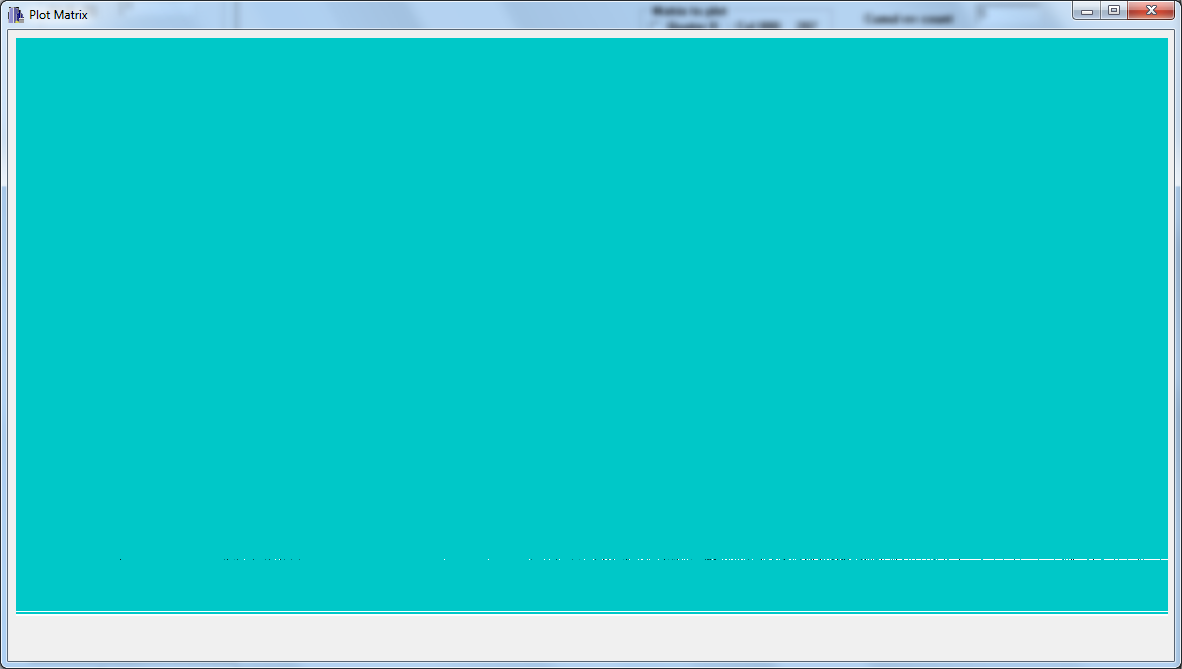
\includegraphics[width = 12cm]{Pictures/Chip3/discri_0.png}
        \label{fig:discri0_chip3}
        \caption{Discriminators output for thresholds set to 0. There is a line not working properly (pixels closed).}
      \end{center}
    \end{figure} 

    \item Discriminators calibration:
    \begin{center}
    \begin{tabular}{ M{1.3cm} M{1.3cm} M{1.3cm} M{1.3cm} M{1.3cm} M{1.3cm} M{1.3cm} M{1.3cm} M{1.3cm} }
      \hline %-------------------------------------------------------------------
      \rowcolor{light-gray} $V_{ref1_A}$ START  & $V_{ref1_B}$ START & $V_{ref1_C}$ START & $V_{ref1_D}$ START & $V_{ref2}$ & $V_{ref1_A}$ STOP & Step & Event nb / step & Number of Runs \tabularnewline
      \hline %-------------------------------------------------------------------
      \hline %-------------------------------------------------------------------
       84  &  117  & 117  & 95  &  98  &  140  &  2  &  500  &  29  \tabularnewline
      \hline %-------------------------------------------------------------------
    \end{tabular}
    \end{center}
 
    \item Temporal noise, fixed pattern noise and offset:

            \begin{center}
              \begin{tabular}{ c c c c }
                \hline %----------------------------
         \rowcolor{light-gray}         Matrix  &  TN   &  FPN  &  Offset  \tabularnewline
                \hline %----------------------------
                \hline %----------------------------
                    A     & 0.990 & 0.375 &  0.304    \tabularnewline
                \hline %----------------------------
                    B     & 0.984 & 0.293 & 0.580   \tabularnewline
                \hline %----------------------------
                    C     & 0.997 & 0.543 & 0.579   \tabularnewline
                \hline %----------------------------
                    D     & 0.969 & 0.344 &  0.882    \tabularnewline
                \hline %----------------------------
              \end{tabular}
            \end{center}
    
    \item Estimation of the fake hit rate ("middle points" thresholds + 20 uadc): $9.69 10^{-6}$ hits/frame/pixels. 
    
    \end{itemize}

    \subsubsection{2}

    The chip was disconnected from the flex.

    \subsubsection{1}

    \begin{itemize}
  
    \item Estimation of the "middle points":
    \begin{center}
    \begin{tabular}{ c c c c c }
      \hline %-------------------------------------------------------------------------------------
      \rowcolor{light-gray} $V_{ref_2}$  &   $V_{ref_{1A}}$  &   $V_{ref_{1B}}$  &   $V_{ref_{1C}}$  &   $V_{ref_{1D}}$  \tabularnewline
      \hline %-------------------------------------------------------------------------------------
      \hline %-------------------------------------------------------------------------------------
      98        &        121        &          97       &       77         &       146        \tabularnewline
      \hline %-------------------------------------------------------------------------------------
    \end{tabular}
    \end{center}
 
    \begin{figure}[!h]
      \begin{center}
        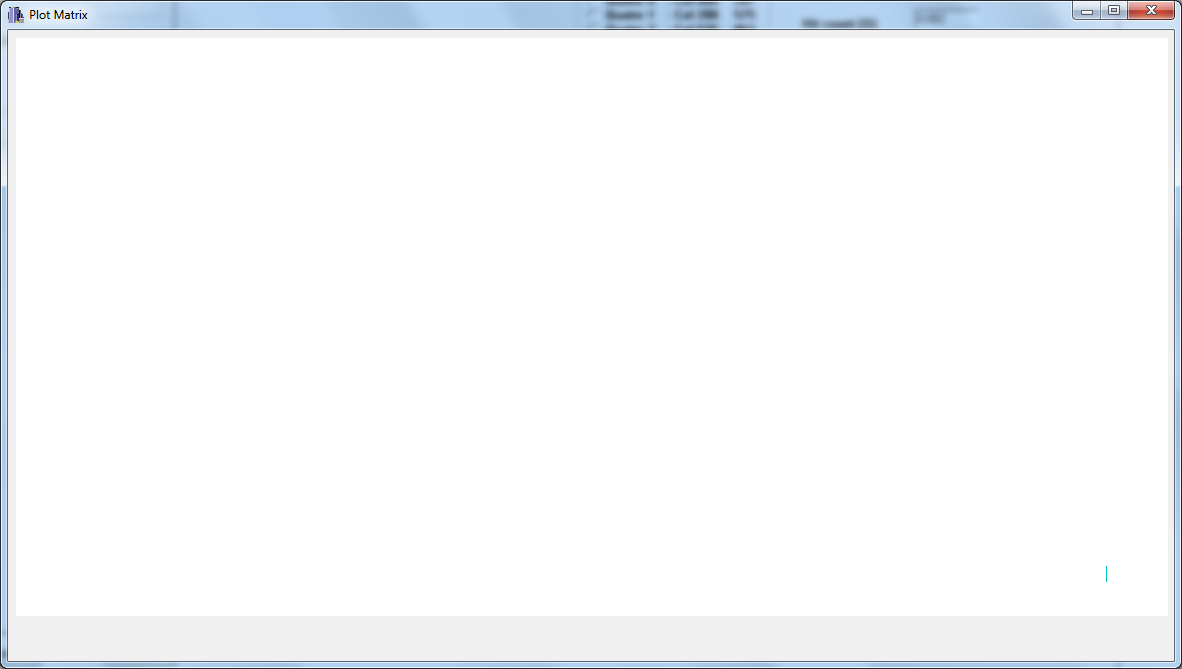
\includegraphics[width = 12cm]{Pictures/Chip1/discri_255.png}
        \label{fig:discri0_chip1}
        \caption{Discriminators output for thresholds set to 255. There is a column (few lines) on submatrix D which is opened.}
      \end{center}
    \end{figure}
   
    \item Discriminators calibration:
    \begin{center}
    \begin{tabular}{ M{1.3cm} M{1.3cm} M{1.3cm} M{1.3cm} M{1.3cm} M{1.3cm} M{1.3cm} M{1.3cm} M{1.3cm} }
      \hline %-------------------------------------------------------------------
      \rowcolor{light-gray} $V_{ref1_A}$ START  & $V_{ref1_B}$ START & $V_{ref1_C}$ START & $V_{ref1_D}$ START & $V_{ref2}$ & $V_{ref1_A}$ STOP & Step & Event nb / step & Number of Runs \tabularnewline
      \hline %-------------------------------------------------------------------
      \hline %-------------------------------------------------------------------
       93  &   69  &  49  & 118 &  98  &  149  &  2  &  500  &  29  \tabularnewline
      \hline %-------------------------------------------------------------------
    \end{tabular}
    \end{center}
 
    \item Temporal noise, fixed pattern noise and offset:

            \begin{center}
              \begin{tabular}{ c c c c }
                \hline %----------------------------
         \rowcolor{light-gray}         Matrix  &  TN   &  FPN  &  Offset  \tabularnewline
                \hline %----------------------------
                \hline %----------------------------
                    A     & 1.054 & 0.407 &  0.397    \tabularnewline
                \hline %----------------------------
                    B     & 1.037 & 0.269 & 0.677   \tabularnewline
                \hline %----------------------------
                    C     & 1.039 & 0.598 & 1.046   \tabularnewline
                \hline %----------------------------
                    D     & 1.053 & 0.543 &  1.005    \tabularnewline
                \hline %----------------------------
              \end{tabular}
            \end{center}
    
    \item Estimation of the fake hit rate ("middle points" thresholds + 20 uadc): $4.67 10^{-5}$ hits/frame/pixels. 
    
    \end{itemize}

  \section{Fake Hit Rate}
\end{document}
